\section{熱系(中村・坂本)}

\subsection{熱設計の方針}
熱系については,下記の考え方のもと設計・検証を実施した.この考え方は主に,戸谷剛・北海道大学准教授がふくい宇宙産業創出研究会WGで講演(2016年11月24日)された資料をご厚意で見せていただき,そこからの学びを元に構築した.
\begin{itemize}
	\item 温度が均一化できるところをなるべく増やし,複雑度を下げる方針とした.
	\item Thermal Desktop等解析ソフトを用いた詳細解析は行わず,解析については少数節点解析でのパラメータサーベイのみを行った.結果,当初設計の表面仕上げで良いとの見込みのもと開発を進めた.
	\item 受動的熱制御を主体とした.ただし,開発の最後のフェーズでバッテリにヒータを貼付し,能動的熱制御を取り入れる設計変更をした.
	\item 材料の熱光学パラメータは宇宙科学研究所小川研のご厚意で,TESA2000を使用させていただき計測した.
	\item 接触コンダクタンスの影響を少なくするため熱伝導シートを導入した.
	\item ウェルリサーチ社の熱真空槽を用い,熱平衡試験でパラメータ同定をしたのちに,熱真空試験で機器の動作確認をした.これらの試験については別章に記載する.
\end{itemize}

下図のように節点へ分割したモデルを作成した.Matlabを用いin-houseでプログラムを書いた.
\begin{figure}[H]
	\centering
	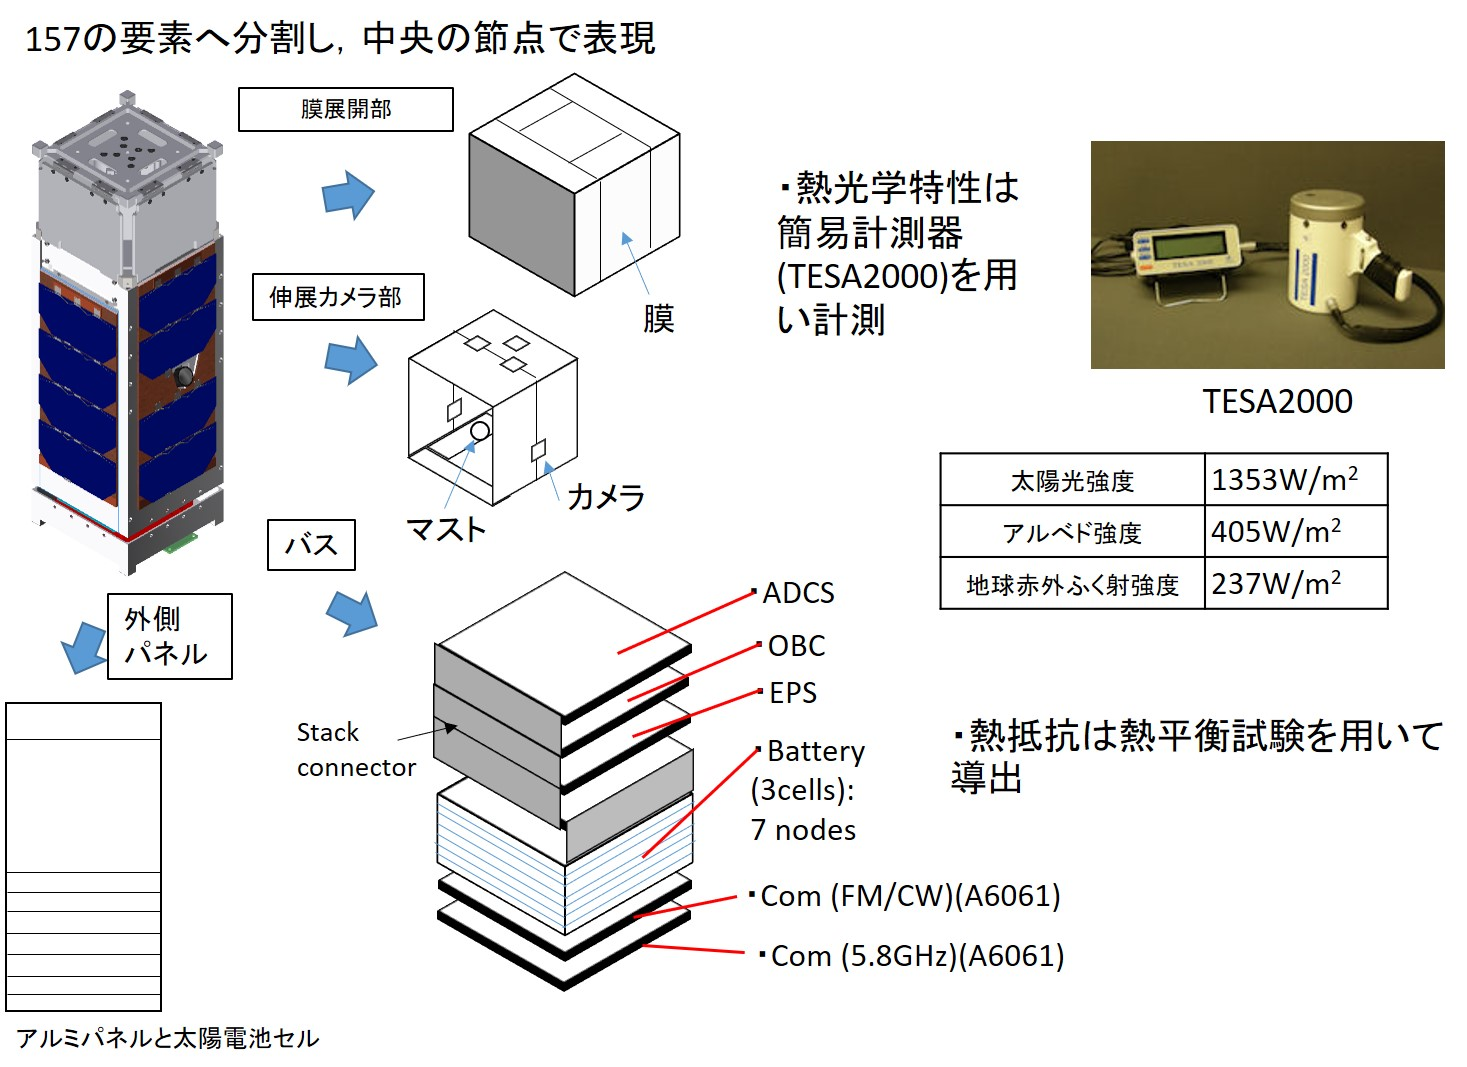
\includegraphics[width=0.8\textwidth]{03/fig/3-7-1.jpg}
	\caption{節点法による熱解析}
	\label{fig3-7-1}
\end{figure}

パラメータ同定のために熱平衡試験を実施した.試験については別章にて詳説する.概要を数に示す.
\begin{figure}[H]
	\centering
	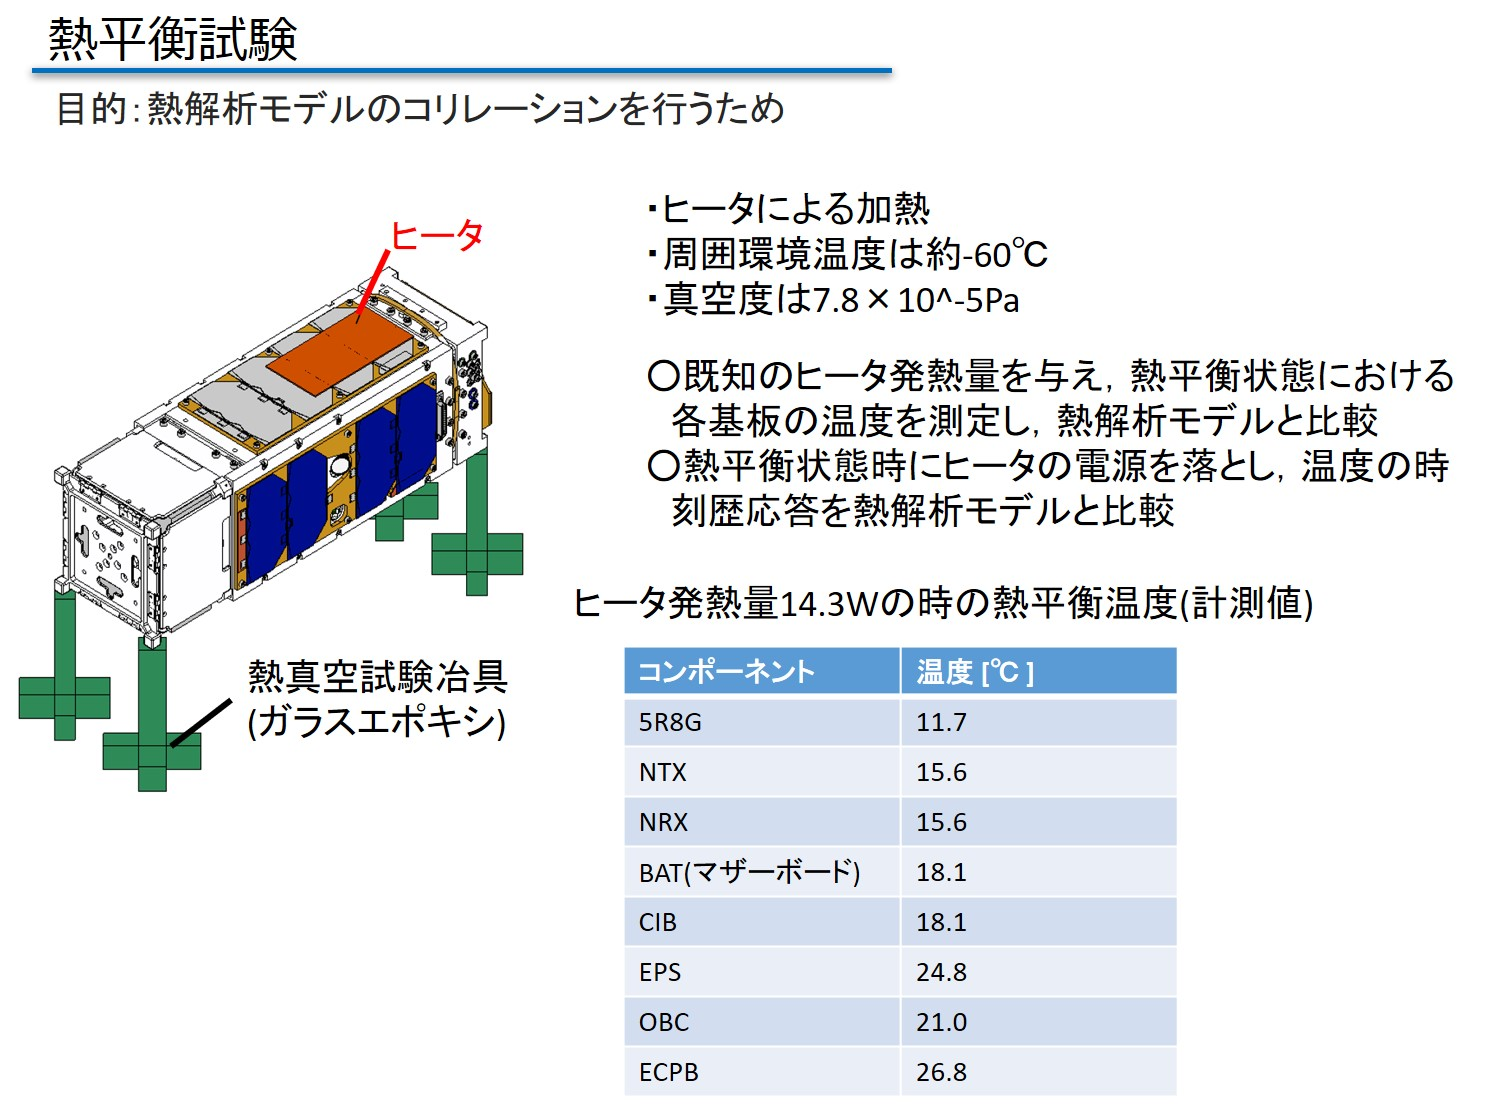
\includegraphics[width=0.8\textwidth]{03/fig/3-7-2.jpg}
	\caption{熱平衡試験による解析モデルコリレーション}
	\label{fig3-7-2}
\end{figure}
ここで得たパラメータを元に,節点解析モデルを用いて,軌道上での各節点の温度変化を予測した.

\subsection{熱解析結果:高温ケース}
高温ケースで以下の結果を得た.
\begin{figure}[H]
	\centering
	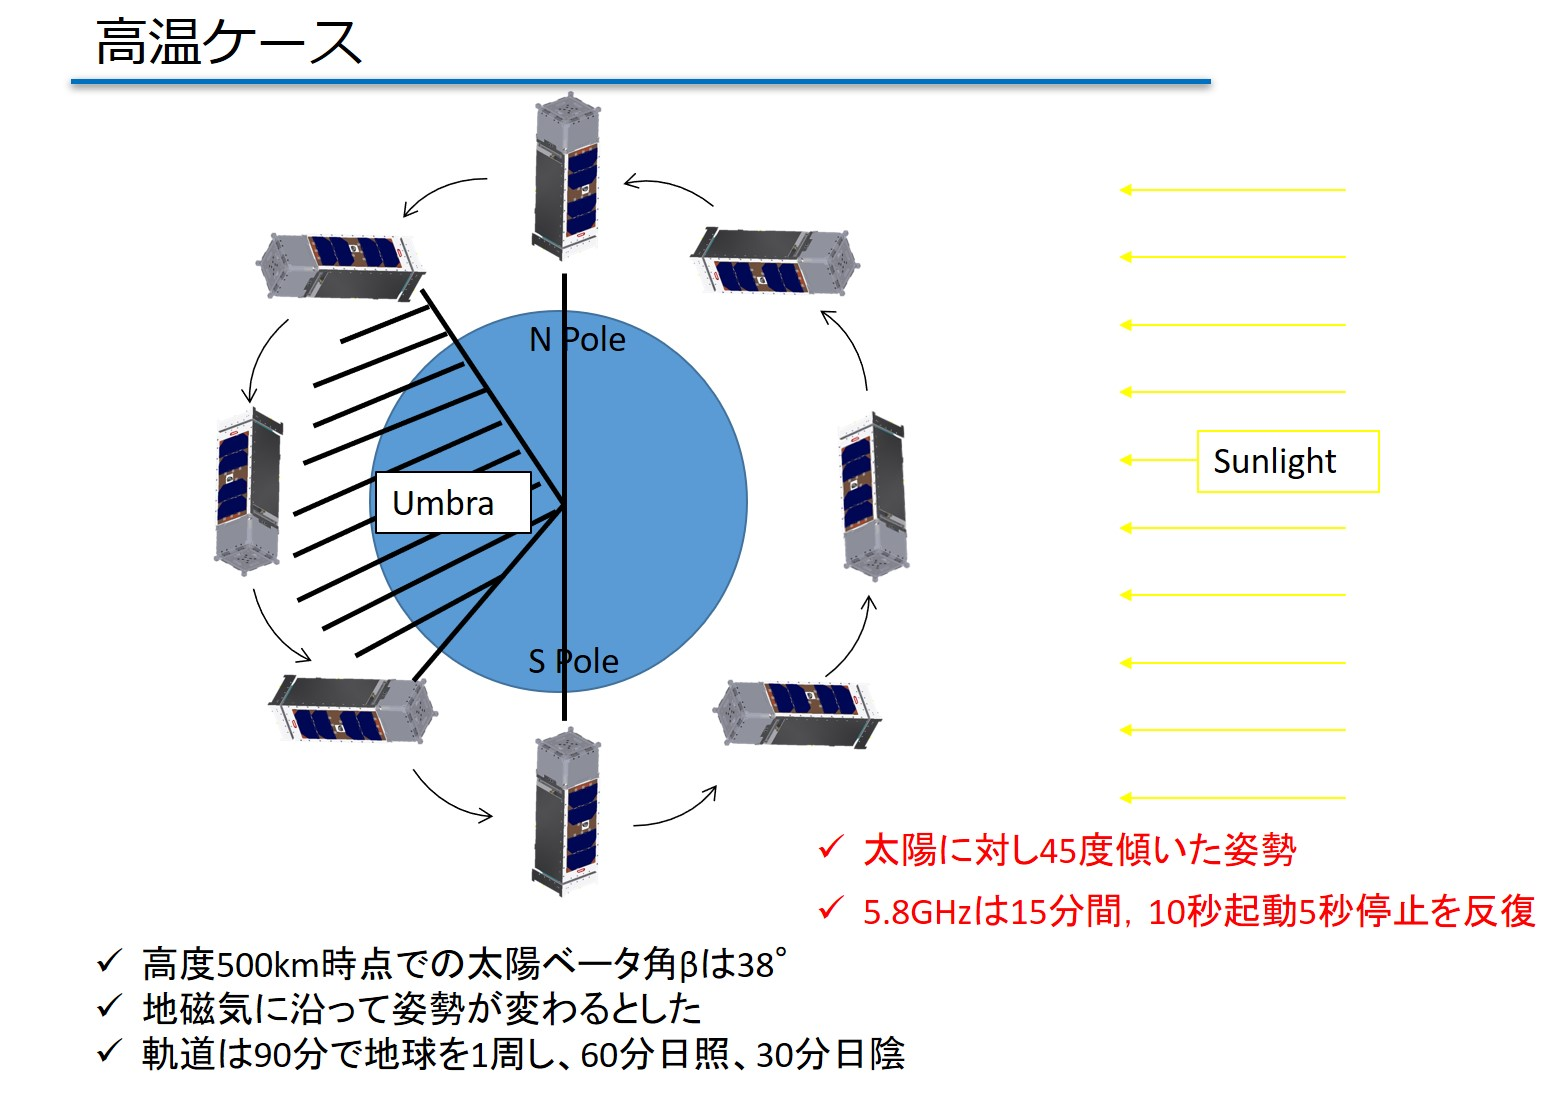
\includegraphics[width=0.5\textwidth]{03/fig/3-7-3.jpg}
		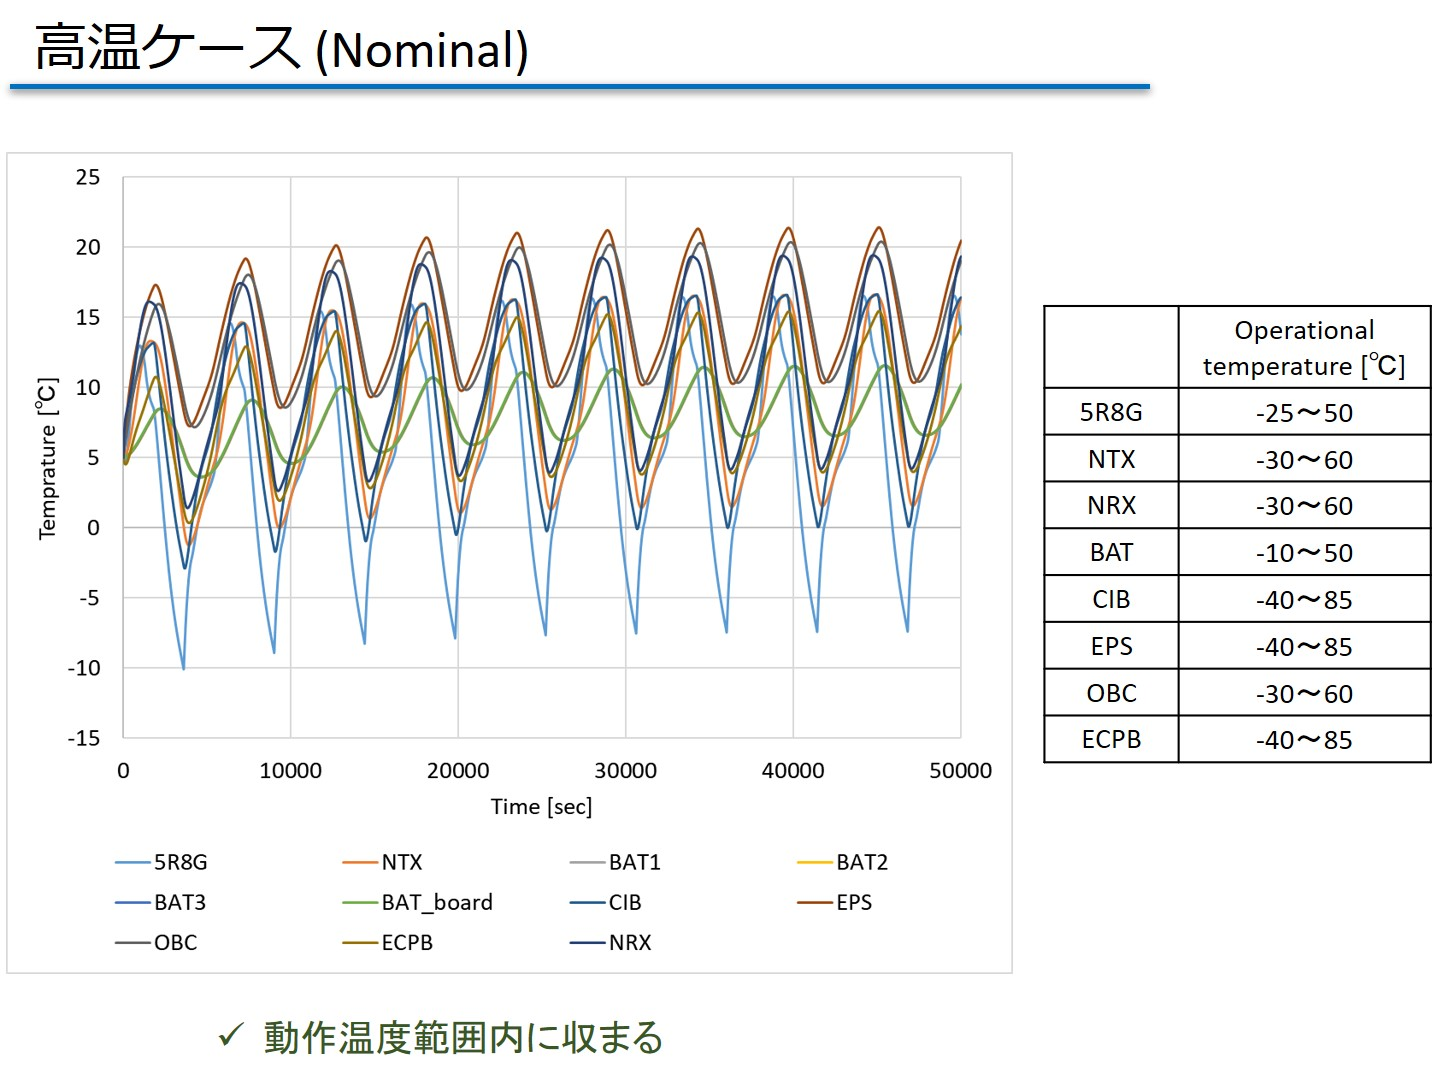
\includegraphics[width=0.5\textwidth]{03/fig/3-7-4.jpg}
				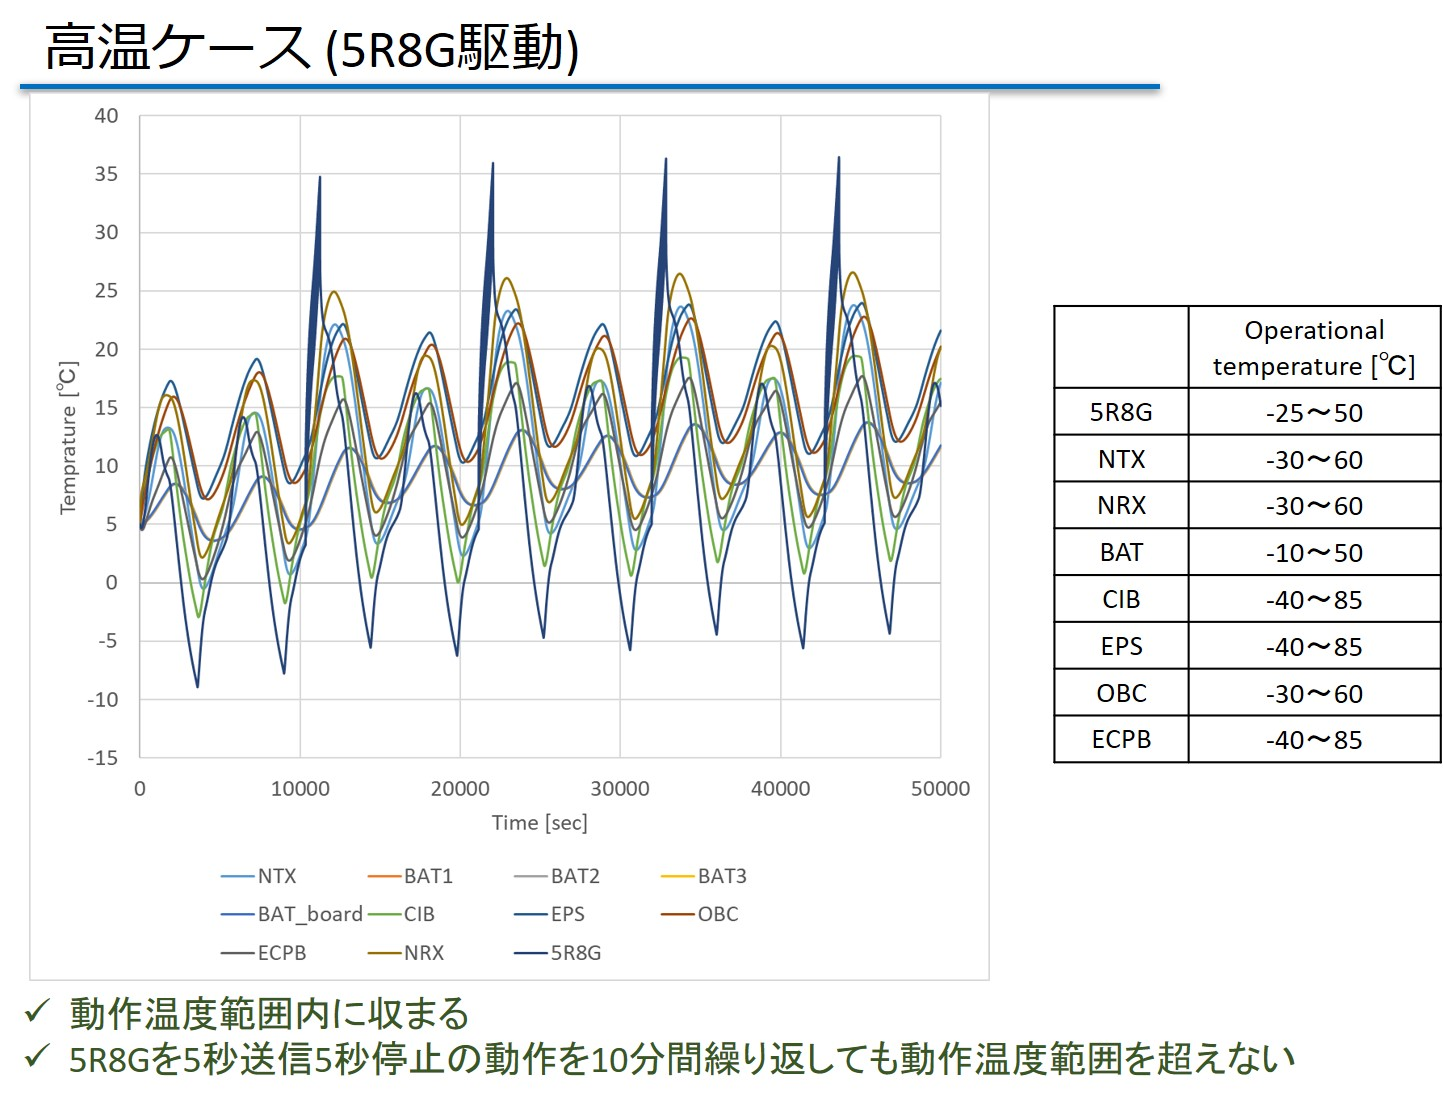
\includegraphics[width=0.5\textwidth]{03/fig/3-7-5.jpg}
	\caption{節点法熱解析結果:高温ケース}
	\label{fig3-7-3}
\end{figure}

\subsection{熱解析結果:低温ケース(Nominal)}
膜展開前の低温ケースで以下の結果を得た.
\begin{figure}[H]
	\centering
	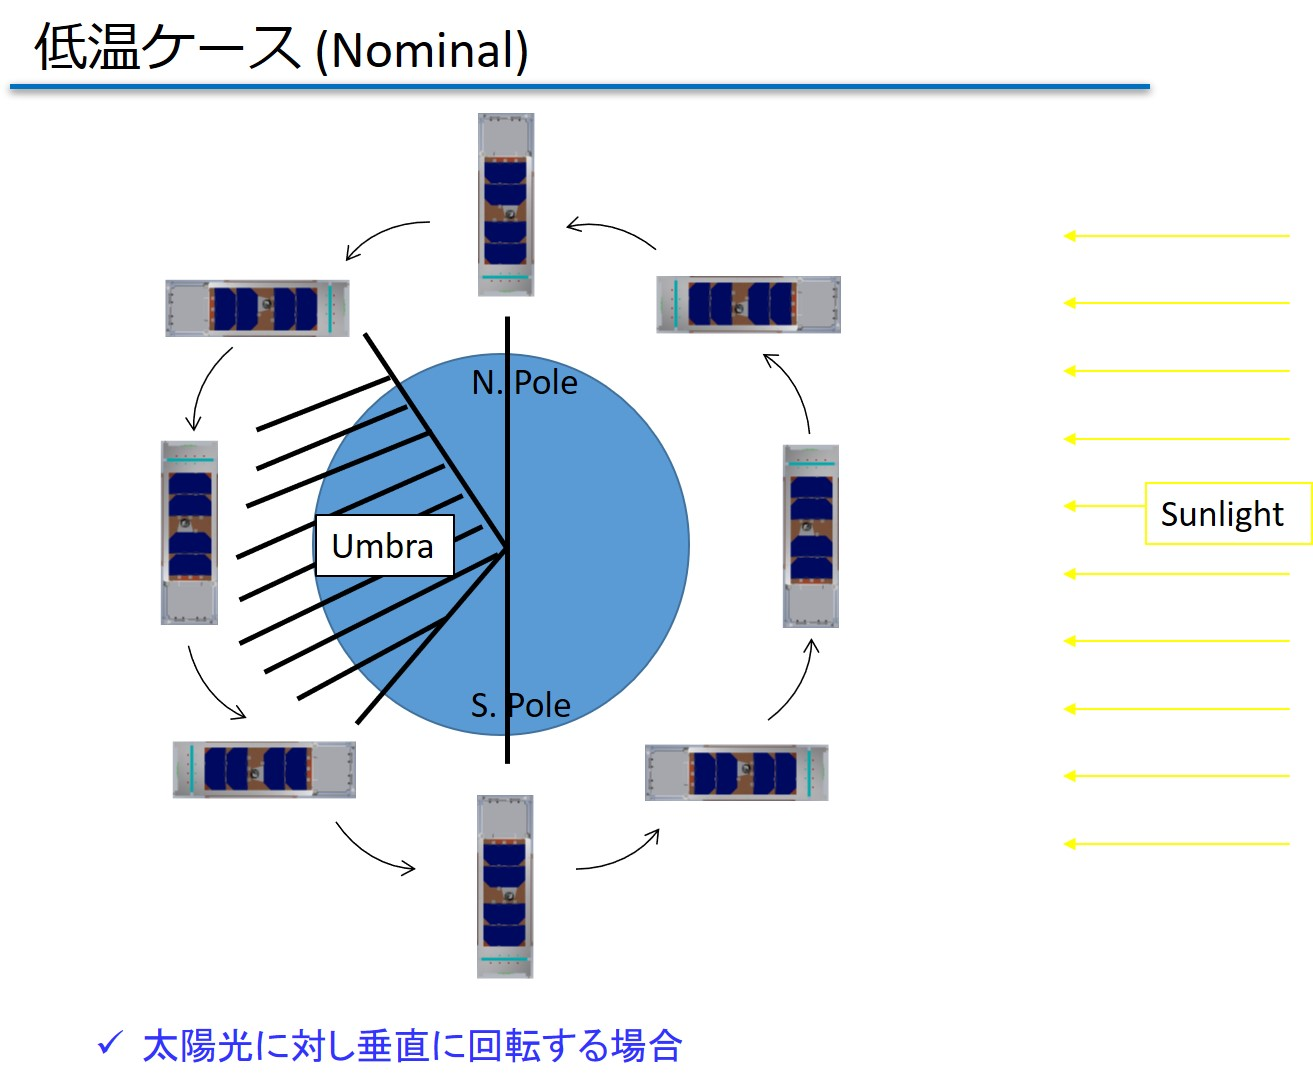
\includegraphics[width=0.8\textwidth]{03/fig/3-7-6.jpg}
	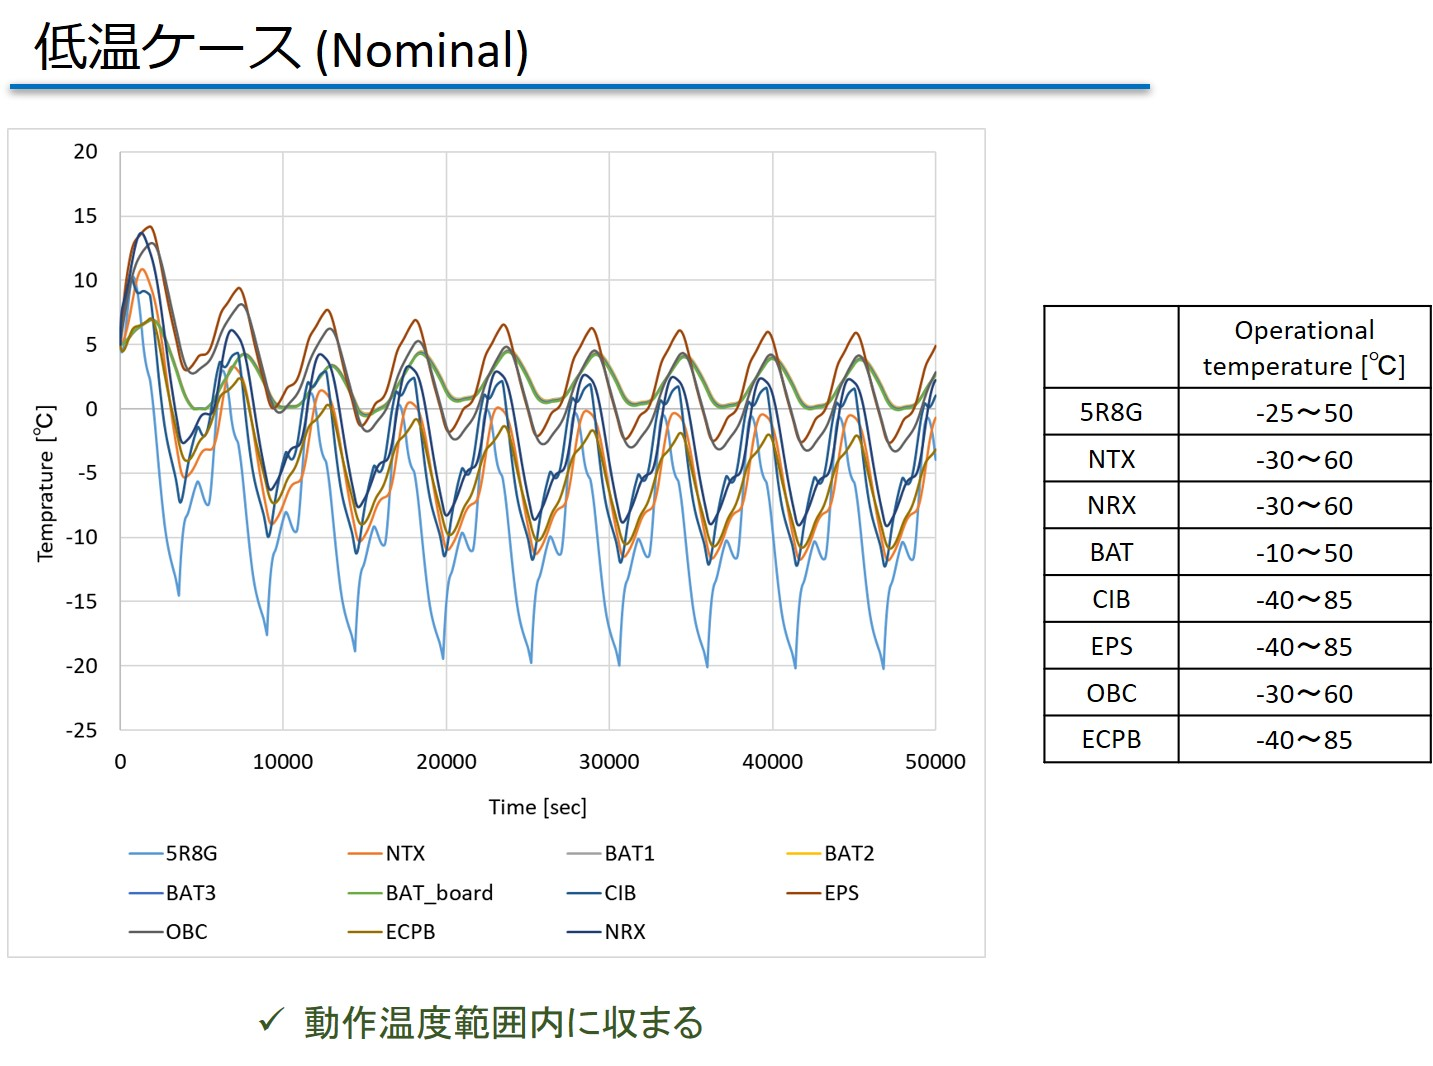
\includegraphics[width=0.8\textwidth]{03/fig/3-7-7.jpg}
	\caption{節点法熱解析結果:低温ケース(Nominal)}
	\label{fig3-7-6}
\end{figure}

\subsection{熱解析結果:低温ケース(膜展開後)}
膜展開後の低温ケースで以下の結果を得た.
\begin{figure}[H]
	\centering
	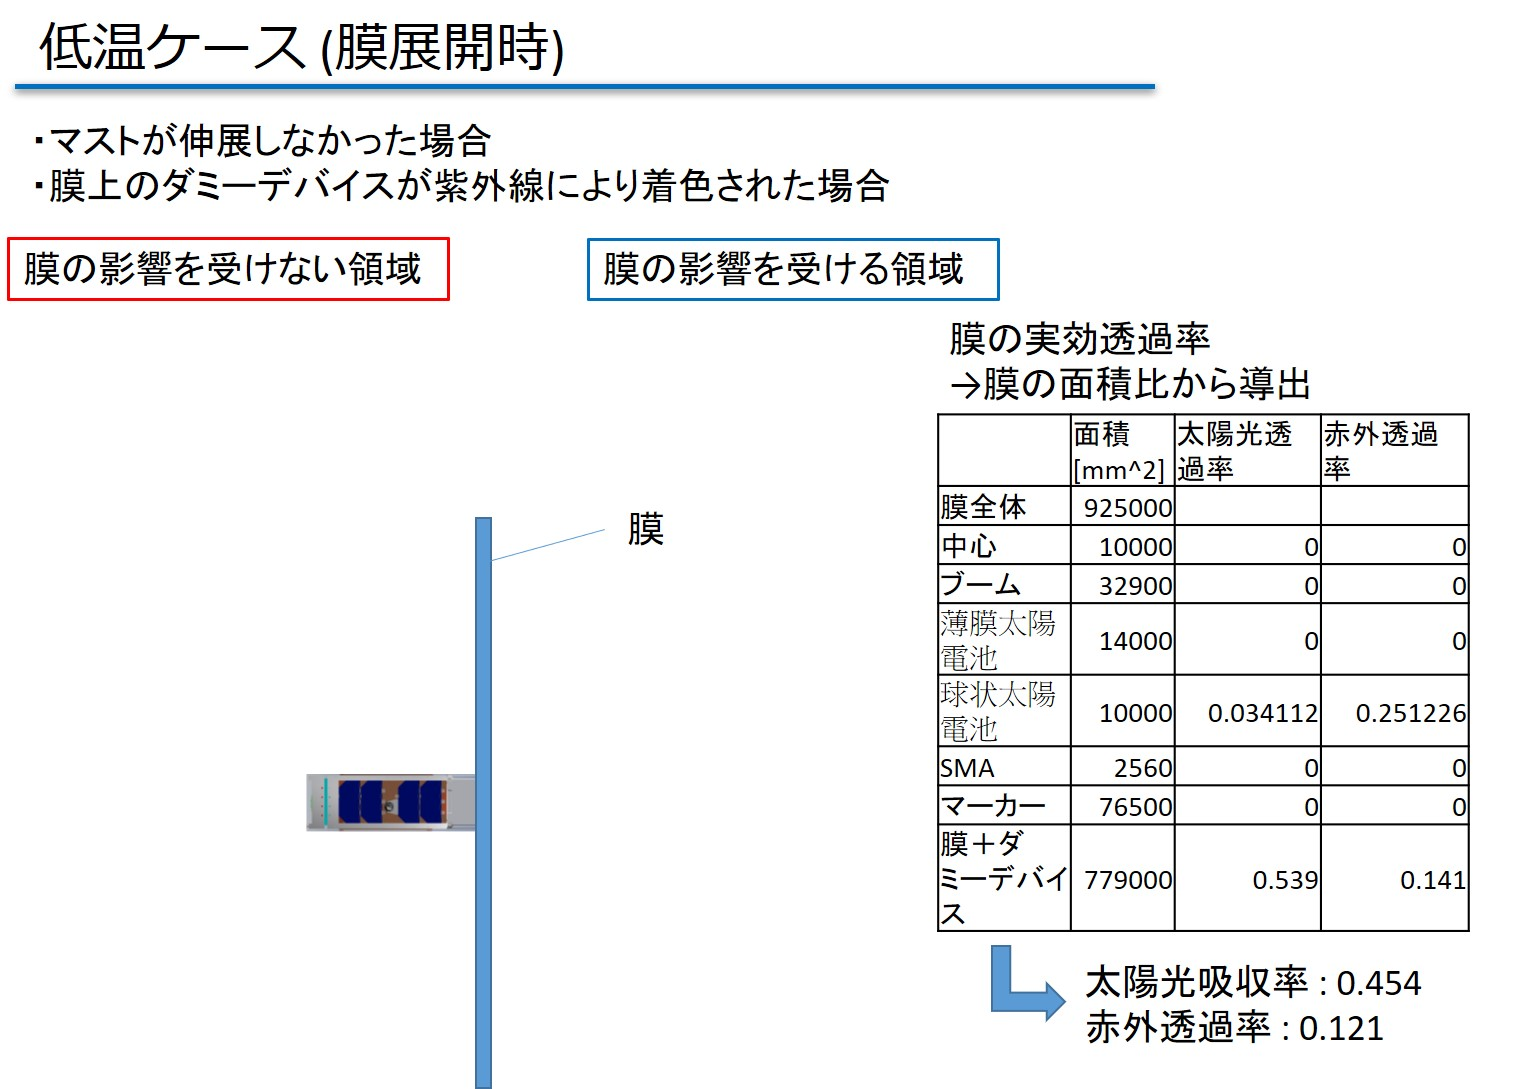
\includegraphics[width=0.8\textwidth]{03/fig/3-7-8.jpg}
	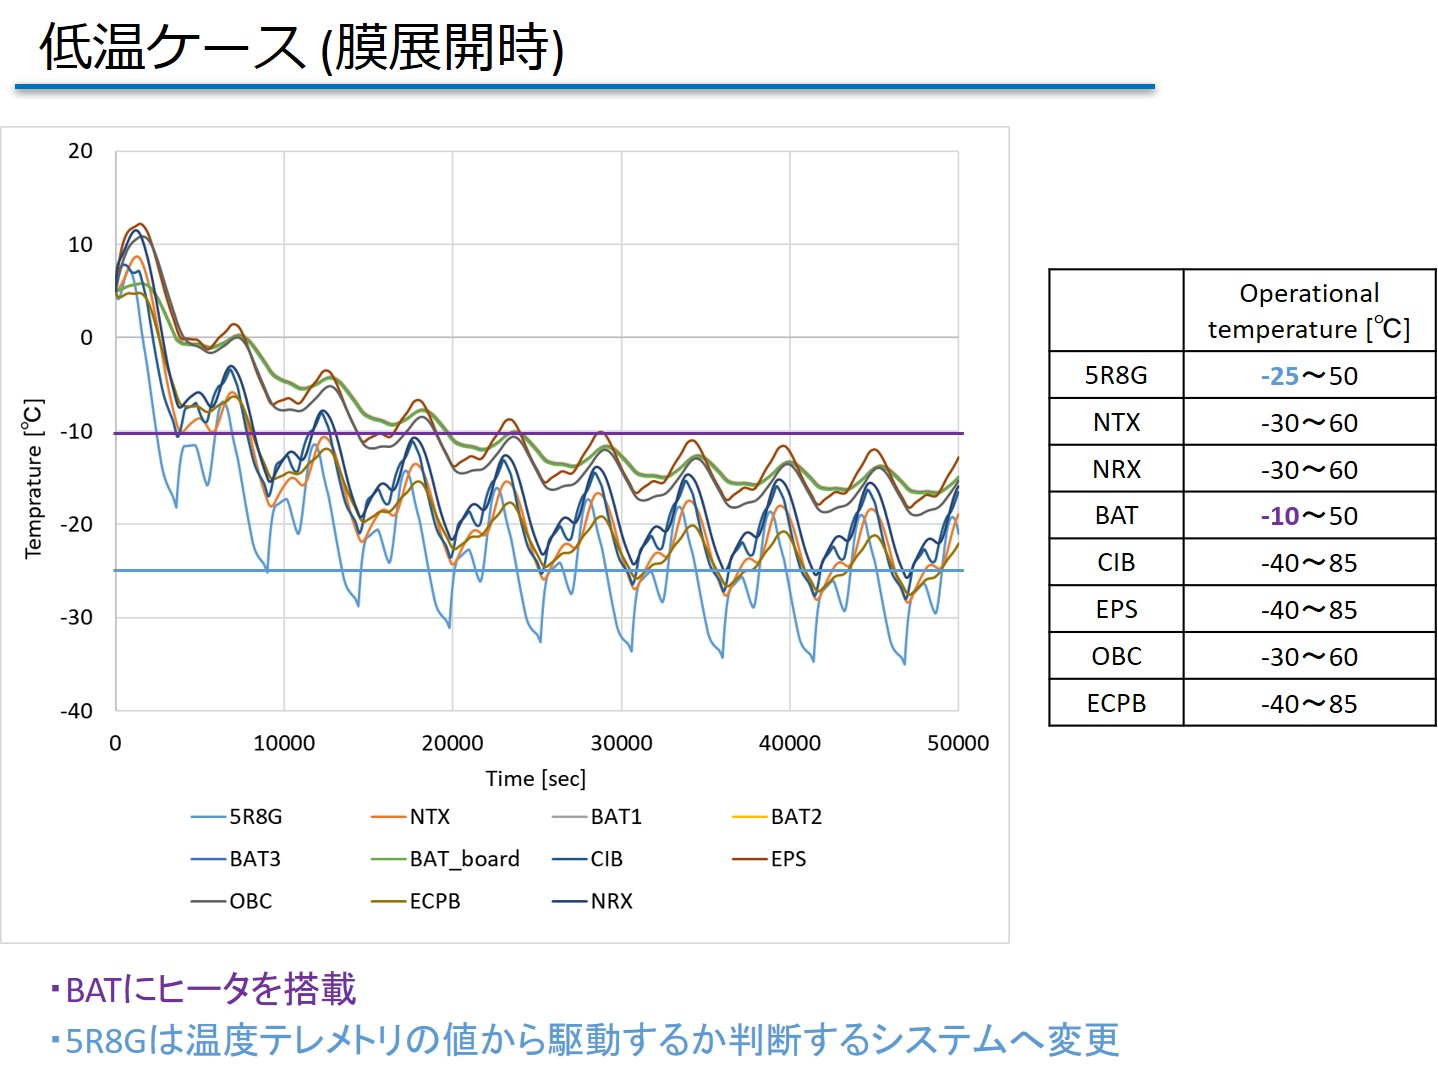
\includegraphics[width=0.8\textwidth]{03/fig/3-7-9.jpg}
	\caption{節点法熱解析結果:低温ケース(膜展開後)}
	\label{fig3-7-8}
\end{figure}

\subsection{熱系の振り返り}
別章に掲載する軌道上温度のHKデータを見ると,解析結果よりも温度が高く,また温度変化の幅も小さい.したがって解析・実験による予測が適切でなかった可能性がある.
軌道上結果を見る限りでは,バッテリにヒータを追加する設計変更は不要だった可能性がある(ただし膜を展開していないので膜展開時についてはさらなる詳細解析を要する).
